%%% Local Variables:
%%% mode: latex
%%% TeX-master: "../main"
%%% End:

\chapter{外文资料的书面翻译}
\label{cha:engorg}
\begin{center}
在快速近似近邻查询中选取近邻候选集最高效的方法是什么?
\end{center}
\section{摘要}
近似近邻查询是一项被广泛运用于许多应用场景中的基础而重要的技术。它主要包括两个阶段:选择近邻候选集合和在候选集合进行最朴素的暴力搜索。只有第一个阶段有提升的空间。在现有的大部分方法中,大多是通过将空间近似量化。计算查询数据与被量化的数据(如聚类中心或者比特序列)之前的距离,然后选择适当大小的候选集。这类方法准确性的衡量就是通过在候选集合度量计算来实现。这看似合理但却忽略了一个重要的问题:没有考虑到选取过程的计算时间代价。在本文中,我们提出一种新的近似近邻查询方法,同时关注选取候选集过程的代价。现有的一些方法都用到一些代价比较大的技术,比如说排序或者堆,但我们提出的方法并非如此,是一种非常高效的检索方法。在 $ 10^8$ 的 SIFT 特征数据检索上,相比于现有最好的方法,我们成功减少了 $1/3$ 左右的计算时间。
\section{简介}
给定一个查询数据,查找出与之相近的数据,这就叫做近邻查询。近似近邻查询是在近邻查询基础上的近似。近似近邻查询问题被主动地研究和广泛地应用于许多场景,如近似重复检测、大规模物体识别、文档检索、光学字符识别。近似近邻查询的特点就是在节省时间和空间地情况下准确地找出真正的近邻候选集。在本文中,我们关注于计算效率与准确率之前的关系。

下面我们来讨论一下近邻查询问题中查询准确率与计算时间之前固有关系。如果不考虑计算时间,那么近邻查询问题可以用暴力枚举的方法解决,直接计算查询数据与原有数据之间的距离。因此耗时太长,这种朴素的解决方法并不实用,特别是在处理大数据集时。减少计算时间其实就是要减少最终暴力枚举的数据量。我们先选出一个小的近邻候集合,在这个数据集上进行暴力枚举。只有在选取候选集合的过程需要我们去优化时间效率和准确率。在选取候近邻选集合时,近邻候选集越大,最终查询的准确率就越高,但是这样就会使得最终暴力枚举的时间变长。

目前已有的大多数方法都是通过衡量候选集合的准确性来衡量算法的性能。候选集合的大小决定了暴力枚举的计算时间。然而,选取近邻候选集的过程的计算时间是独立的。因此,忽略掉选取候选集合时间的做法只是觉得了近似近邻查询问题的一部分。

有些文章也适当地考虑了计算时间代价问题。在他们当中,最有效的方法就是多重倒排索引(inverted multi-index,IMI)。然而,在”选取近邻候选集最高效的方法是什么?“这一问题上,我们发现这个问题没有抓住选择近邻候选集过程的本质。下面我们直观上来解释下,假设有 $n$ 个数据,任务是选取近邻候选集,集合大小为 $k$($k<n$)。最差的方法就是将他们全部排序,这需要耗时是$O(n\log n)$。一种更好的方法就是采用有限队列对他们部分排序。这样,每一条数据都被加入到优先队列当中,最终 $k$ 个最近邻的数据留下了。这需要的时间就是 $O(n\log k)$。多重倒排索引用的就是这种方法。然而,还有一种更快的排序方法——桶排序。因为不需要比较序数,它可以在 $O(n)$ 时间复杂度内完成。因此,如果我们能够选择合适的桶,那么选取近邻候选集的过程就可以加快。我们的目标是选取出近邻候选集,所以我们没有必要对桶内的元素按照距离去排序。

对于大规模数据的近似近邻查询问题,我们提出了一种比以往更加高效的近似近邻查询方法。提出的这种方法称为桶距离哈希(bucket distance hashing, BDH)。在实验中,我们在相同平台上比较了这种方法与几种代表性的近似近邻查询方法,分别比较了召回率与计算时间的关系以及召回率与候选集合大小的关系。虽然我们的目标的解决近邻查询问题,但是同样的方法也可以运用到 k 近邻搜索问题当中。
\section{相关工作}
要想高效地选取近邻候选集,通常需要先将数据进行索引。按照索引结构的不同,近似近邻查询方法可以被分为基于树的方法和基于哈希的方法。基于哈希的方法同时也分为数据无关和数据相关两类。前者在索引的过程中不会使用原始数据而后者需要使用。
\subsection{基于树的方法}
FLANN 是一种基于树索引的代表方法。它可以自动选择随机 kd-树,层次 k-means 和暴力枚举中一种最优的方法以及在给定数据集上调参。在实验过程中,我们会将随机 kd-树和层次 k-means 与我们的方法进行比较。
\subsection{基于哈希的数据无关方法}
局部敏感哈希(locality sensitive hashing,LSH)是一种代表性的基于哈希的数据无关的方法。近年来也有很多人对其进行改善。然而众所周知它的性能比数据相关的索引方法要差。此外,拒局部敏感哈希比数据相关的方法也要执行速度上也要慢很多。
\subsection{基于哈希的数据相关方法}
数据相关的方法可以分为在欧氏空间和汉明空间进行选取近邻集合两种。
\textbf{在欧氏空间中选取} \\

这种方法通常使用量化和数据压缩的技术。向量量化(vector quantization,VQ)应用到近似近邻查询中,例如 VQ-index 和 IVFADC。乘积量化(product quantization)被运用在 IMI 当中。正如前面所提到的,IMI 方法要比 IVFADC 方法的效果更好。转换编码被应用在 [3] 中。这一过程可以看做是标量量化(scalar quantization,SQ)。在这个类别中,我们选取 IVFADC 和 IMI 进行比较评价,二者会在下一章节中再介绍。虽然我们实现转换编码,但是它无法和二者比较。
\textbf{在汉明空间中选取}\\

这种方法中,数据通常用二进制编码表示。由于位运算 XOR 操作,这样可以减少内存占用和在汉明空间中的距离计算时间。由于这些好的特性,许多近似近邻查询方法都是基于二进制编码的。在他们当中,谱哈希(spectral hashing,SH)就是一种代表性的方法。

为了实现高召回率的长编码,编码长度为 128 比特或者 256 比特是比较常见的。其实处理这么长的编码是不简单的。在汉明空间中选取近邻候选集合的基准方法是顺序查找。这种方法虽然很快,但却无法再大数据集上应用。有人也许认为树结构或哈希结构能够实现子顺序查找。然而,在汉明空间进行等距离数据的查找,随着距离增大,查找的数据量会呈现出爆炸增长。这使得选取近邻候选集的过程变得不太高效。正如 [16] 中之处一样,使用原始的 LSH 来哈希。然而前面提过,数据无关的方法并不高效。另一个也许稍微复杂一点的方法就是现有的在欧氏空间的近似近邻查询方法。我们将自己提出的方法运用在谱哈希上。但是,并没有将其与现有的代表性方法进行比较。
\section{现有基于向量和乘积量化的哈希方法}
回顾一下 IVFADC 和 IMI 方法可以帮助更好地理解我们提出的方法 BDH。因此在这一章节,我们会比第二章中更加详细介绍他们。
\subsection{IVFADC}
IVFADC 使用 VQ 索引数据可以高效地选取近邻候选集,使用 k-means 聚类算法将数据分成许多个聚类。给定一个查询数据,与之相近的聚类会被检索到,隶属于该聚类的所有数据会被选为近邻候选集。这有可能使得有些数据与查询数据近邻却没有被选取到近邻集合中。然而在相同聚类中心数量下的量化误差最小,VQ 被认为是最好的量化方法。
\subsection{多重倒排索引}
作为比 IVFADC 更好的解决方法,Babenko 和 Lempitsky 提出的 IMI 使用乘积量化代替向量量化。PQ 是一种介于 SQ 和 VQ 之间的量化方法。向量空间被划分成很多个子空间,之后再每个子空间上运用 VQ 编码。在相同数量的聚类中心下,PQ 一般会产生比 VQ 更大的量化误差。然而为了达到相同召回率,计算时间可以通过多序列算法(MSA)来减少。
\begin{figure}[H]
  \centering
  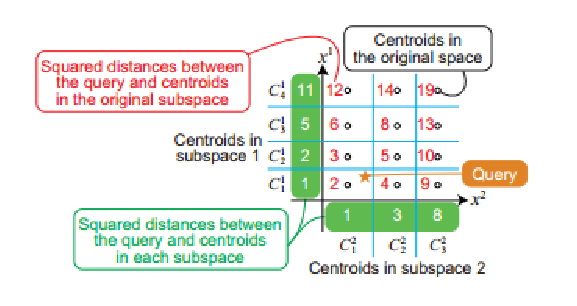
\includegraphics[width=0.5\linewidth]{f_imi}
  \caption*{IMI 算法的介绍}
  \label{fig:f_imi}
\end{figure}
上图中回顾介绍了 IMI 算法。根据图片所示,在子空间 1 中有 4 个聚类中心,在子空间 2 中有 3 个聚类中心。聚类中心的用 $C_j^i$ 表示,其中 $i$ 表示子空间标号,$j$ 表示第 $i$ 个子空间中的聚类标号。首先,计算用星号表示的查询数据与子空间聚类中心之间的平方距离。原始的平方距离是每个子空间中的平方距离之和。然后,如果在原始空间中的所有距离都计算完了,中心离查询数据近的就会被查找出。但是,没有必要去计算在原始空间中所有的距离。因为子空间中的中心距离大的中心并不能在过程中发挥作用。因此,他们在 MSA 算法中被忽略不计。
\begin{figure}[H]
  \centering
  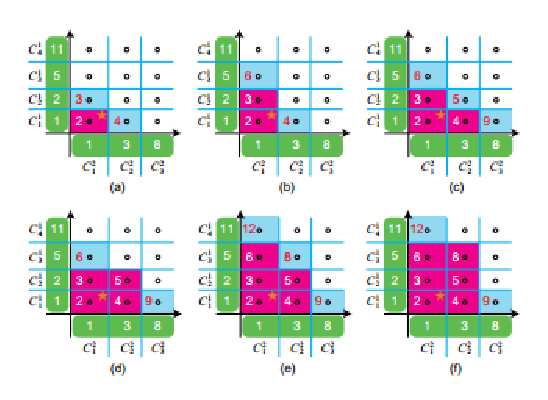
\includegraphics[width=0.5\linewidth]{f_msa}
  \caption*{MSA 算法的介绍}
  \label{fig:f_msa}
\end{figure}
图中是 MSA 算法的概览。在 MSA 算法中,每个子空间中的平方距离事先被排序好了。然后,子空间的中心按距离递增顺序一次排列。正如 图(a)所示,第一个查找的聚类就是 $C_1^1 \times C_1^2$ 的积,与查询数据的距离为 2。相邻的聚类中心 $C_2^1 \times C_1^2$ 和 $C_1^1 \times C_2^2$ 会在下一次中作为候选集被查找出。

如上所示,MSA 算法比较聚类中心之间的距离并将其按照升序排列。这在近邻查询中是不必要的。在这点上,这种方法就没有抓住近邻查询的本质。图中描述了子空间数量为 2 的情况。如果空间划分多于 2 的话,那么整个计算的代价就会变大。因此,IMI 算法最佳情形就是子空间数量为 2。我们将会展示子空间被划分成多余 2 同时获得更好的查询效率的算法。
\section{提出的方法}
\subsection{回顾}
正如第一章节中所提,我们提出的方法最关键的想法就是在选取近邻候选集的时候不做数据的排序。我们采用分支定界法来代替 MSA 算法解决相同问题。
\begin{figure}[H]
  \centering
  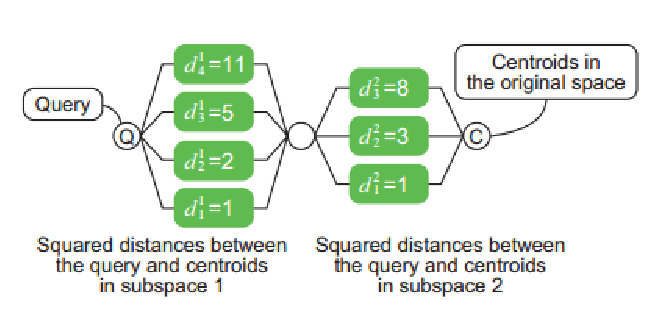
\includegraphics[width=0.5\linewidth]{f_distance}
  \caption*{子空间的距离计算}
  \label{fig:f_distance}
\end{figure}
图中,介绍了我们所提出的算法。图中绘制了查询数据(Q)和聚类中心(C)路径。路径的左右半边分别表示在查询数据和聚类中心之间子空间 1 和子空间 2 中的平方距离 $\{d^i_j\}$。$d^i_j$ 和 $C^i_j$ 的标号示意相同。然后,我们会确定平方距离的上界。整个过程中,上界会不断地增大。在所有路径中,距离小于上界的聚类中心就会被查找出来。
\begin{figure}[H]
  \centering
  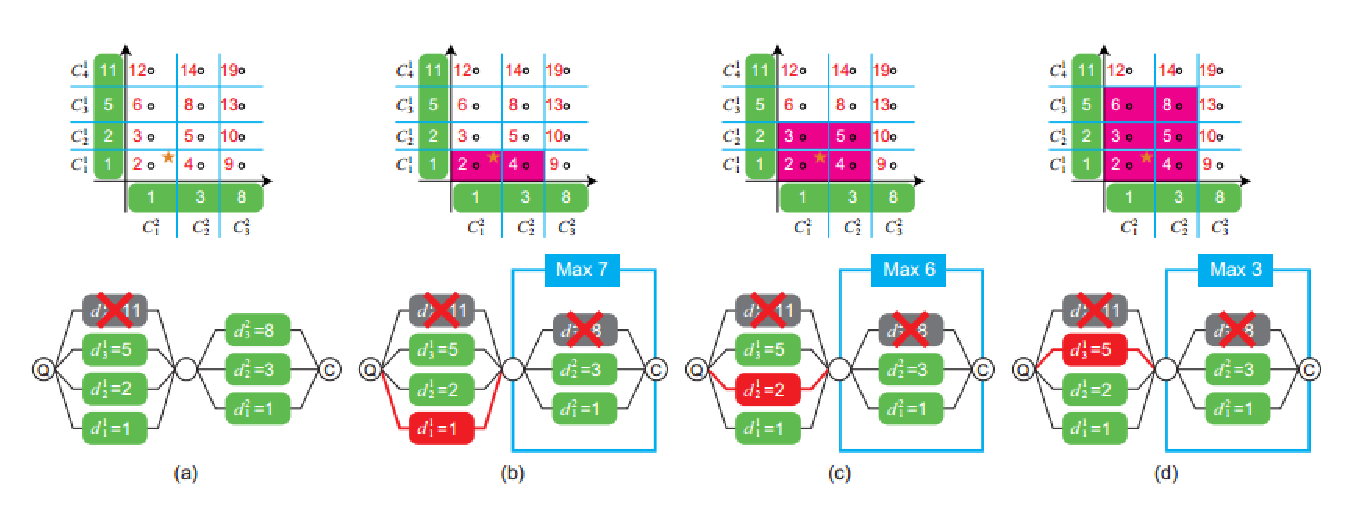
\includegraphics[width=\linewidth]{f_bdh}
  \caption*{BDH 算法示意图}
  \label{fig:f_bdh}
\end{figure}
图中描述了提出的算法流程,平方距离的上界是 8。整个算法流程从(a)到(d)。在(a)中,当上界被设置成 8,路径 $d^1_4 =11$ 就会立即被删除。之后,子空间 1 中的每条路径都会遍历一遍。在(b)中,路径 $d^1_1$ 被遍历。由于上界是 7,路径上子空间 2 中 $d^2_1 =1$ 和 $d_2^2=3$ 会被选出到近邻候选集。在(c)中,$d^1_2$ 被遍历,由于上界是 6,路径上子空间 2 中 $d^2_1 =1$ 和 $d_2^2=3$ 会被选出到近邻候选集中。
\subsection{准备}
为了更详细地解释我们提出的方法,需要提前做一些定义。我们假设,查询数据 $q$ 和待查询数据集都用向量表示。用 $N$ 和 $D$ 分别表示待查询数据的数量和维度。我们会在待查询数据集上进行 PCA 降维以减小距离度量的误差和获取最大的 $u$ 个主成分(特征值)降序的 $l_1,l_2,\ldots,l_u$。用$\mathbf{V}=[v_1 v_2 \cdots v_u]$ 表示与 $u$ 个特征值对应特征向量组成的矩阵。$u$ 对应多维哈希表的维度。我们之后会介绍一种自动确定 $u$ 大小的算法。
\subsection{索引与调参}
PQ 将特征空间划分成 $p$ 维的子空间。例如,一个 $u$ 维的向量 $\mathbf{x}$ 被 $u$ 个特征值表示为 $\mathbf{x} = \{x_1,\ldots,x_m\}$,其中 $m = u/p$。然后,在 $p$ 维的子空间上进行 k-means 聚类。

除去 $p$ 以外,我们提出一套自动调参的算法。首先,我们开始为聚类算法进行自动调参选择。目标是要将待查询数据集在第 $i$ 个子空间聚类成 $k_i$ 个类,得到所有 ${k_i}$ 以及每个子空间中的聚类中心。用$x_{is}$表示第 $s$ 条数据的第 $i$ 个子向量,用 $C_j^i$ 表示第 $i$ 个子空间中的第 $j$ 个聚类中心。然后量化误差第 $i$ 个子空间的$E_i$定义如下:
\begin{equation*}
E_i = \sum_{s=1}^N\left( x_{is} - C^i_{q_i(x_{is})}\right)^2
\end{equation*}
其中 $q_i(x)$ 函数定义如下:
\begin{equation*}
q_i(x) = \arg\min_{j} \left( x - C^i_j\right)^2
\end{equation*}
因为过大的量化误差会导致距离度量时的误差过大,所以我们要采取策略使得子空间中的 $E_{max}$ 最小。算法 1 介绍了我们提出的算法。它会增加具有最大量化误差的子空间中聚类中心的数量,并在当桶的总数量达到待查询数据的数量时结束。这样,特征空间就会被分成 $N_{bkt}$ 个桶,对应到多维哈希表的哈希大小。通过对人造数据和真实数据的实验中,我们可以找到算法的终止条件。

这个算法同时也可以确定多维哈希表的维度 $u$。如果在子空间 1 中有 $k_i$ 个聚类中心,那么子空间中的量化误差就小于 $E_{max}$。假如子空间不需要划分,假设特征值被降序排列,对于 $i=1,\ldots,m'$,现有的 $m'$ 满足 $k_i > 1$ 而且对于 $i=m'+1,\ldots,\lfloor D/p\rfloor$ 有 $k_i=1$。然后可以忽略后半部分($i>m'+1$),$u$ 设置为 $m'p$。
\subsection{高效选取近邻候选集合}
用 $c$ 表示近邻候选集的集合大小。我们提出的算法可以一步一步地选择至少 $c$ 个最近距离的候选数据。算法 2 和算法 3 展示了整个详细过程。其中有一部分在章节 4.1 中已经有所介绍了。算法 2 可以找到距离在下界 $L$ 和上界 $U$ 之间的桶。$L$ 和 $U$ 的初始值分别是 0 和 查询数据与最近桶之间的平方距离。只要当前选取的近邻候选集大小 $n$ 小于 $c$,整个过程会一直循环执行。$\Delta$ 表示 $L$ 和 $U$ 的增量,我们设置 $\Delta$ 的大小为特征值之和的 $1/100$。
\section{实验}
我们通过实验对比提出的方法(BDH)与一些代表性的近似近邻查询算法,包括 IVFADC 和 IMI。所有方法都用 C++ 语言实现。我们依照 MATLAB 版本的 IVFADC 和 C++ 源码 IMI 算法实现基于哈希的方法。 IVFADC、IMI 和 BDH 共用大部分的代码。这样可以避免在实验过程中的差异并且尽可能公平地对比。对于基于树的方法,我们使用 C++ 源码实现的 FLANN。FLANN 自身无法使用于大数据集合。我们通过实验探索每种方法的最佳参数设置。实验中的参数设置见表格。
\begin{table}[htbp]
  \centering
  \caption*{实验中的参数设置}
  \label{tab:f_parameters}
  \begin{minipage}[t]{\linewidth}
    \begin{tabular}{|c|c|c|c|c|c|c|c|}
      \hline
        Methods  & 参数 & SIFT1M& SIFT10M& SIFT100M& GIST1M&GIST10M\\
      \hline
      BDH  &  $\log_2|C|,P$& 20,5 & 26,3 & 28,5 & 22,5 & 24,5\\
      \hline
      IMI  &  $\log_2|C|$  & 14 & 18 & 20 & 18 & 22\\
      \hline
   IVFADC  &  $\log_2|C|$  & 10 & 12 & 14 & 12 & 14\\
    \hline
      RKD  &  $No.of trees$& 8  &  8 &  8 &  8 & 16\\
      \hline
      HKM  &  $k$          & 32 & 64 &  N & 64 & 32\\
      \hline
    \end{tabular}
  \end{minipage}
\end{table}
我们使用包含 10 亿个 128 维 SIFT 特征描述符的 BIGANN 数据集和包含大约 8 亿 384 维 GIST 特征描述符的 80 Million Tiny Images。对于前者,我们使用 1M、10M、100M 大小的数据集,1000 个向量用来做查询。对于后者,我们使用 100K、1M、10M 大小的数据集。对于两类数据,都是用最小的数据集来做训练。

我们使用有 4 CPUs(AMD Opteron 6174,2.2GHz,12 cores)和 256G 内存的服务器来运行实验。所有的数据都存储在内存当中。所有的程序都是单核单线程执行。
\subsection{实验 1:召回率与计算时间}
我们通过召回率与计算时间关系比较了所有的算法。计算时间是平均一次查询所需要的计算时间。由于计算时间限制,计算时间少的准确率相比之下比较低。图中显示了在 SIFT 和 GIST 数据集上的实验结果。从实验结果看出,我们提出的方法比其他方法的效果都要好很多。其中图(c) 中显示在召回率为 90\%时, BDH 算法是 IMI 算法的两倍快,是 IVFDC 的 4.5 快;在召回率为 60\%时,BDH 算法是 IMI 的 2.9 倍快,是 IVFADC 的 9.4 倍快。比较图(a)到图(c),提出的方法的优点随着数据集增大就越明显了。这显示出这个算法的可扩展性好。相反,比较图(d)到图(f),提出的方法的优点并没有变化。

IVFADC 和 IMI 无法扩展是因为相对大规模计算代价。用 $G$ 表示原始空间中的聚类数量, IVFADC 在选择近邻候选集时需要 $O(G)$ 时间来计算距离。IMI 需要 $O(2\sqrt{G})$ 计算距离,需要 $O(\sqrt{G}\log\sqrt{G})$ 在子空间中排序。
\begin{figure}[H]
  \centering
  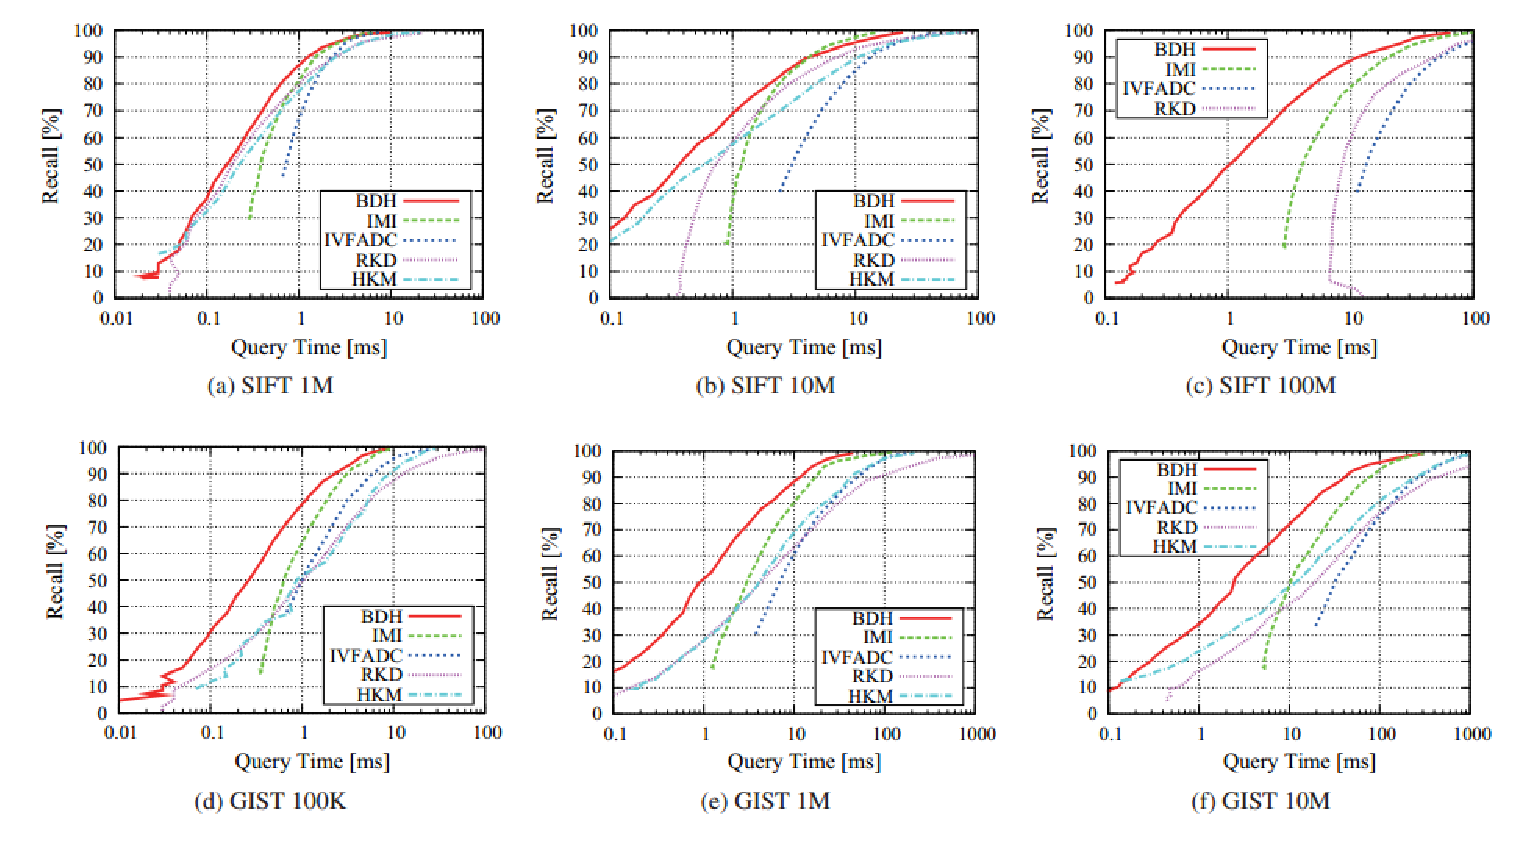
\includegraphics[width=\linewidth]{f_experiments}
  \caption*{实验结果图}
  \label{fig:f_experiments}
\end{figure}
\subsection{实验 2:召回率与候选集大小}
我们同时也通过召回率与候选集大小的关系来比较所有算法。为了适合这个标准,我们选择最佳的参数来进行实验。通过图中可以看到,我们的方法要比 IVFADC 和 IMI 方法好。
\begin{figure}[H]
  \centering
  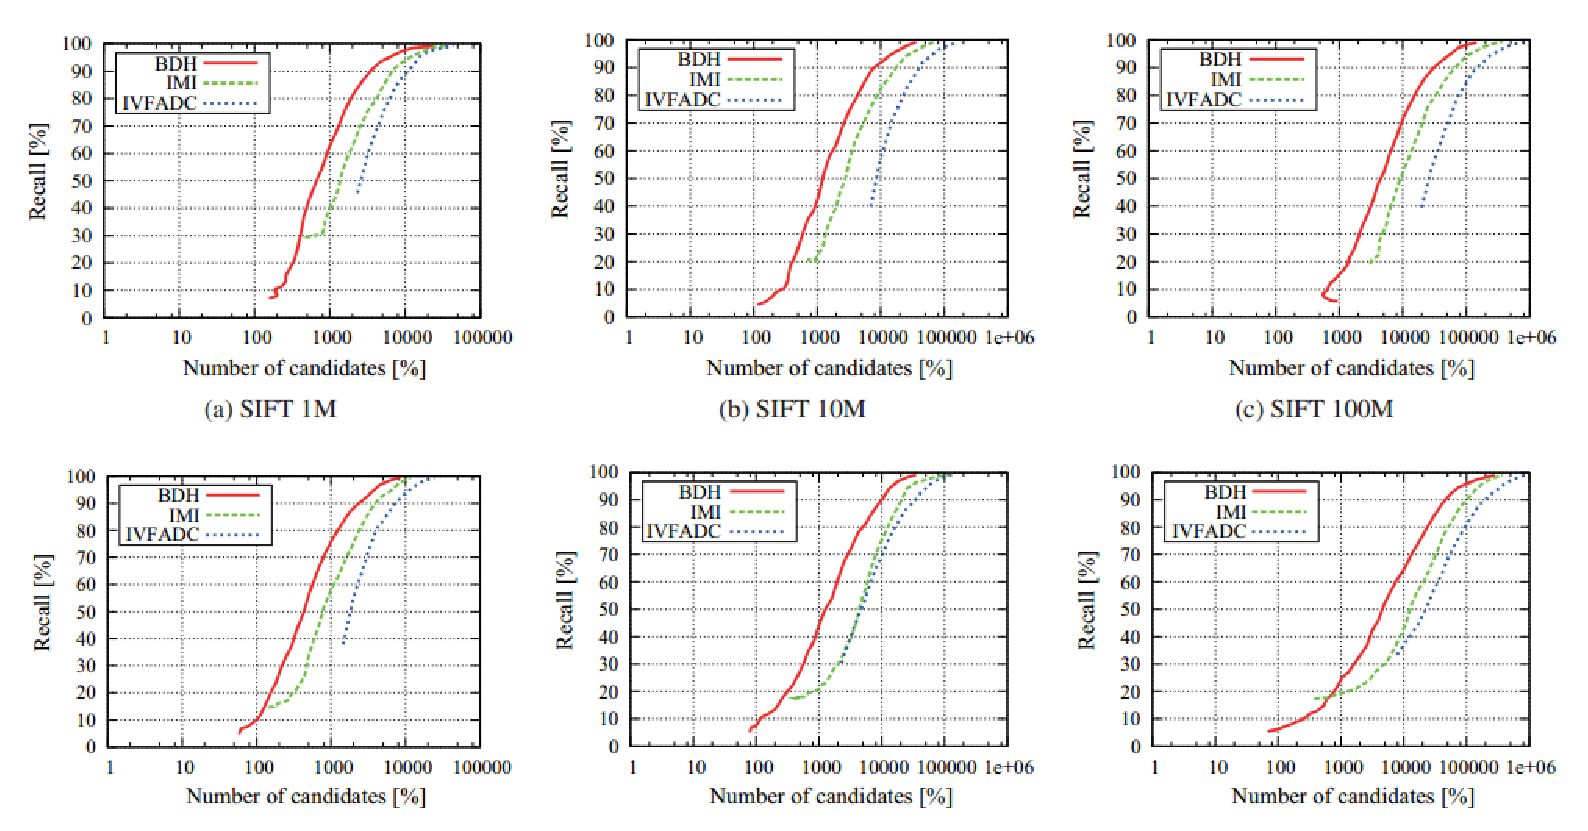
\includegraphics[width=\linewidth]{f_experiments2}
  \caption*{实验结果图 2}
  \label{fig:f_experiments2}
\end{figure}
\section{结论}
在近似近邻查询的过程中,只有选择近邻候选集的过程可以变改善。在本文中,我们指出了衡量近似近邻查询算法的计算代价的重要性。计算代价是近似近邻查询算法的衡量中必不可少,研究者忽略计算时间的方法是有缺陷的。我们发现,目前最好的近似近邻查询算法 IMI 并没有把我到选取近邻候选集合的本质。因为近似近邻查询算法只需要选出最近邻的候选集合,所以没有比较去做排序。

最后,我们提出一种新的将计算代价考虑在内的近似近邻查询算法。这种方法基于分支定界算法,可以进行非常高效地检索。我们也提出一种自动调节参数的算法,除了一个参数以外,其余参数可以自动调节到最好。在 100M SIFT 特征实验中,相比于现有最好的算法,我们提出的算法在减少三分一左右的计算时间。在召回率为 90\% 和 60\% 时,分别是最好算法的 2 倍 和 2.9 倍快。
\begin{center}
\textbf{书面翻译对应的原文索引}
\end{center}

\begin{enumerate}[{$[$}1{$]$}]
\item Iwamura M, Sato T, Kise K. What is the most efficient way to select nearest neighbor candidates for fast approximate nearest neighbor search? The IEEE International Conference on Computer Vision (ICCV), 2013
\end{enumerate}
